\documentclass[a4paper,10pt]{scrartcl}
\usepackage[utf8]{inputenc}
\usepackage[T1]{fontenc}
\usepackage[french]{babel}
\usepackage{textcomp}
\usepackage{array,multirow}
\usepackage{amsmath,amssymb}
\usepackage{amsthm}
\theoremstyle{plain}
\newtheorem{exo}{Exercice}
\usepackage{lmodern}
\usepackage{microtype}
\usepackage{hyperref}\hypersetup{pdfstartview=XYZ}
\usepackage{lmodern}
\usepackage{graphicx}
\usepackage[dvipsnames,svgnames]{xcolor}
\usepackage{microtype}
\usepackage{lipsum}
\usepackage{xcolor}
\usepackage{listings}
\usepackage{fancyhdr}
\usepackage{listings}
\usepackage{url}
\usepackage[T1]{fontenc}
\pagestyle{fancy}
\renewcommand\headrulewidth{1pt}
\fancyhead[L]{ TP 1 NMI}
\fancyhead[R]{univ tln}
\renewcommand\footrulewidth{1pt}
\fancyfoot[R]{\today}
\fancyfoot[L]{Ben Amira}
\usepackage{hyperref}\hypersetup{colorlinks=true,linkcolor=Brown,pdfstartview=XYZ}
\title{\textcolor{teal}{TP 1 NMI}}
\author{\textcolor{darkgray}{Ben Amira Rawia}}
\date{\today}
\begin{document}
\maketitle
\newpage

\begin{exo}
 Rappeler le lien entre l'information mutuelle normalisée I(X,Y) de deux variables aléatoires X et Y et l'entropie de celles-ci.
\end{exo}
L'information mutuelle de deux variables aléatoires est une quantité qui mesure la dépendance entre ces deux variables .
L'information mutuelle normalisée permet de comparer des clusterings ayant des nombres de clusters différents.
L'entropie mesure la quantité moyenne d’information d’un ensemble d’évènements,et son incertitude.

la relation entre entropie et information mutuelle normalisée est : 

\[
\textcolor{teal}{ NMI = \frac{2*MI(C,Y)}{H(C)+H(Y)}}
\]
avec MI : information mutuelle
H(C) : entropie de la premiere variable C
H(Y) : entropie de la deuxieme variable Y 

\begin{exo}
Considérons l'image "lena.jpeg" comme une variable aléatoire, calculer et afficher la densité de probabilité associée
\end{exo}

\centerline{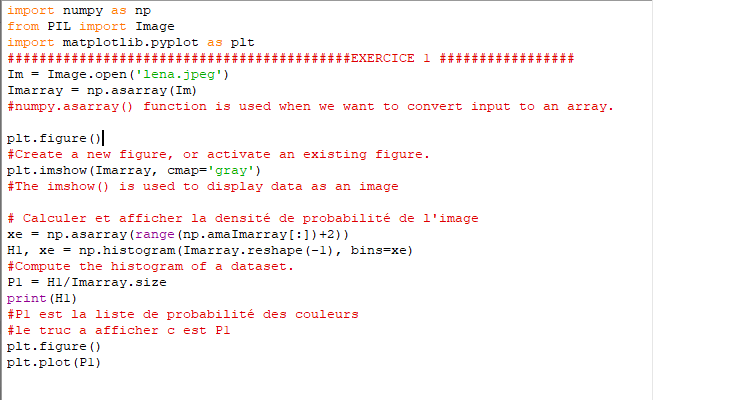
\includegraphics[width=18cm]{hello.png}}

la densite de probabilité est decrite par une matrice geante ( P1)  de 253 elements( ci desoous )

\centerline{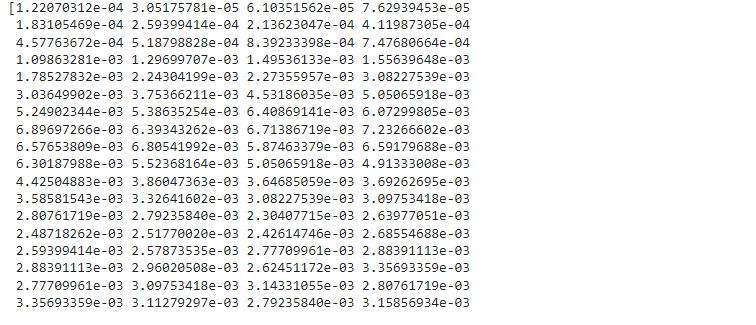
\includegraphics[width=18cm]{p1.png}}


\begin{exo}
Calculer et afficher l'entropie de l'image
\end{exo}

\centerline{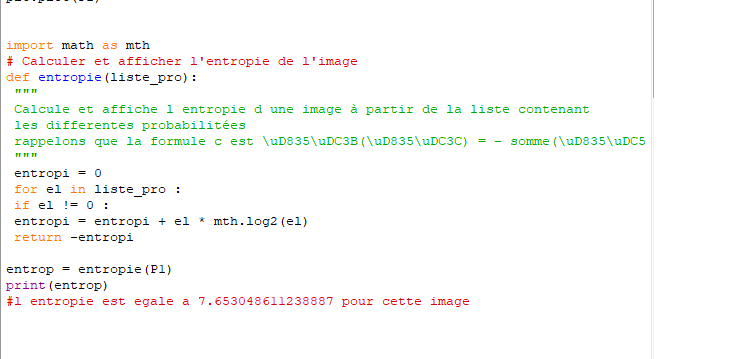
\includegraphics[width=18cm]{hi.png}}

l entropie est egale a 7.653048611238887


\begin{exo}
 Utiliser l'image seuillée lena4 et calculer la densité de probabilité jointe entre lena et lena4 ainsi que l'entropie jointe.
\end{exo}

\centerline{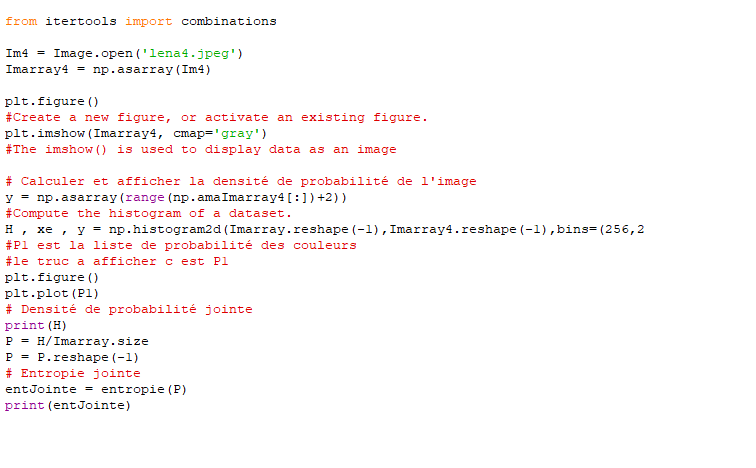
\includegraphics[width=18cm]{bnj.png}}
l'entropie jointe est egale à 10.362911876757801, il suffit de faire appel a la fonction qui calcule l entropie mais avec des valeurs de probabilté jointe qu on extrait grace a la fonction histogram2d


\begin{exo}
Ecrire une fonction NMI(I1, I2) qui renvoie l'information mutuelle normalisée entre les images Im1 et Im2
\end{exo}

\centerline{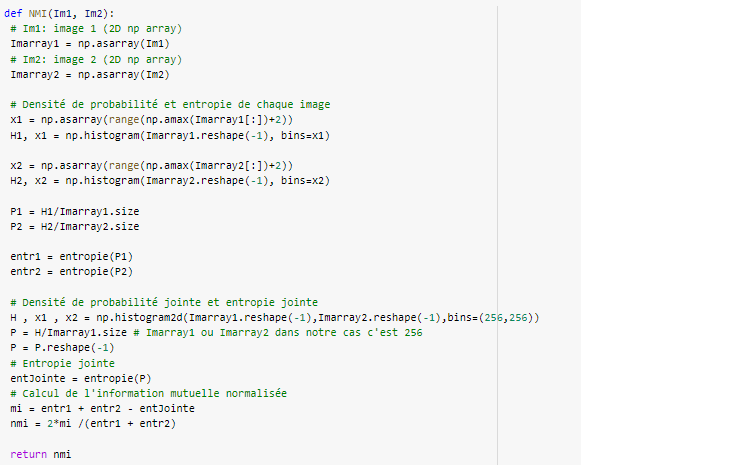
\includegraphics[width=20cm]{sal.png}}
comme on vient de le rappeler dans le premier exercice , le calcule de l information mutuelle normalisé se fait :
\[
\textcolor{teal}{ NMI = \frac{2*MI(C,Y)}{H(C)+H(Y)}}
\]

 
\centerline{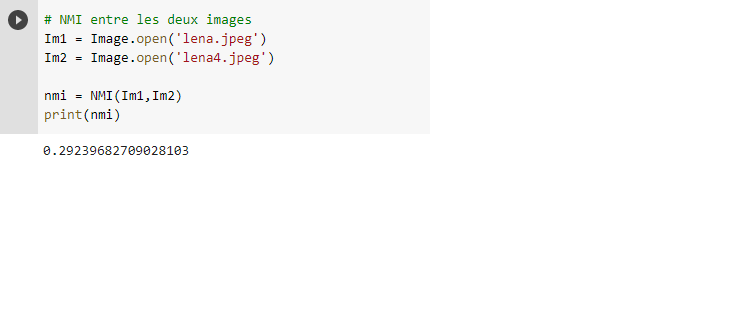
\includegraphics[width=18cm]{sa.png}}



\begin{exo}
On a vu en cours que l'information mutuelle normalisée est maximale lorsque celles-ci sont recalées "au mieux". Ecrire une fonction registration(I1, I2, niter) qui calcule itérativement la translation optimale permettant de registrer les deux images.
\end{exo}

\centerline{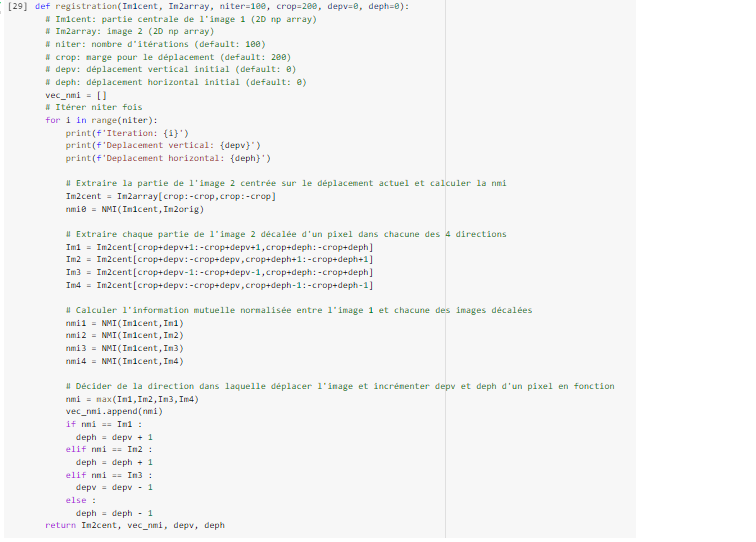
\includegraphics[width=19cm]{say.png}}

l idee de cet algorithme est de partir d une certaine position et de faire des deplacements a chaque fois jusqu'a alignement parfait , arrivée a l alignement parfait l information mutuelle normalisée est maximale donc a chaque essais de depacment horizontale ou verticale , on calcule la NMI entre l image de depart et la nouvelle image deplacé , on compare les 4 NMI calculé pour les 4 sens ( haut , bas , droit gauche ) , la plus grande valeur de NMI sera choisie parmis les 4 , et l image sera deplacé dans le sens qui a la plus grande NMI 



\end{document}